\documentclass[11pt, a4paper]{article}
\setlength{\oddsidemargin}{0.5cm}
\setlength{\evensidemargin}{0.5cm}
\setlength{\topmargin}{-1.6cm}
\setlength{\leftmargin}{0.5cm}
\setlength{\rightmargin}{0.5cm}
\setlength{\textheight}{24.00cm} 
\setlength{\textwidth}{15.00cm}
\parindent 0pt
\parskip 5pt
\pagestyle{plain}
\usepackage{graphicx}
\usepackage{amsmath}
\usepackage{amsthm}
\usepackage{amssymb}
\usepackage{mathrsfs}
\usepackage{fancyhdr}
\usepackage{mathpazo}
\usepackage{microtype}
\usepackage{hyperref}
\usepackage{xcolor}
\usepackage{mdframed}
\usepackage{array}
\usepackage{booktabs}
\usepackage{graphicx}
\usepackage{subfigure}
\usepackage{placeins}
\usepackage{changepage}

\title{Project Proposal}
\author{}
\date{}


\newcommand{\namelistlabel}[1]{\mbox{#1}\hfil}
\newenvironment{namelist}[1]{%1
\begin{list}{}
    {
        \let\makelabel\namelistlabel
        \settowidth{\labelwidth}{#1}
        \setlength{\leftmargin}{1.1\labelwidth}
    }
  }{%1
\end{list}}

\begin{document}
	
\begin{titlepage} % Suppresses headers and footers on the title page
	
	\centering % Centre everything on the title page
	
	\scshape % Use small caps for all text on the title page
	
	\vspace*{\baselineskip} % White space at the top of the page
	
	%------------------------------------------------
	%	Title
	%------------------------------------------------
	
	\rule{\textwidth}{1.6pt}\vspace*{-\baselineskip}\vspace*{2pt} % Thick horizontal rule
	\rule{\textwidth}{0.4pt} % Thin horizontal rule
	
	\vspace{0.75\baselineskip} % Whitespace above the title
	
	{\LARGE Sensor Mesh Network\\} % Title
	
	\vspace{0.75\baselineskip} % Whitespace below the title
	
	\rule{\textwidth}{0.4pt}\vspace*{-\baselineskip}\vspace{3.2pt} % Thin horizontal rule
	\rule{\textwidth}{1.6pt} % Thick horizontal rule
	
	\vspace{2\baselineskip} % Whitespace after the title block
	
	%------------------------------------------------
	%	Subtitle
	%------------------------------------------------
	
	Final Report Draft
	
	
	\vspace*{14\baselineskip} % Whitespace under the subtitle
	
	%------------------------------------------------
	%	Editor(s)
	%------------------------------------------------
	
	By
	
	\vspace{0.5\baselineskip} % Whitespace before the editors
	
	{\scshape\Large \textit{Mike DiDomenico (md848)}  \\} % Editor list
	{\scshape\Large \textit{Kenneth Huaman (khc96)} \\} % Editor list
	{\scshape\Large \textit{Karthik Dasaraju (kd453)} \\} % Editor list
	
		\vspace{2\baselineskip} % Whitespace below the editor list
	
	{\large Project Supervisors: \textit{Prof. Joseph Skovira, Jacob George (Kionix) }} % Publisher
	
	\vspace{0.5\baselineskip} % Whitespace below the editor list
	

	
	\vfill % Whitespace between editor names and publisher logo
	
	%------------------------------------------------
	%	Publisher
	%------------------------------------------------
	
	%\plogo % Publisher logo
	
	\vspace{0.3\baselineskip} % Whitespace under the publisher logo
	
	05/09/2019 % Publication year
	
	{\large Cornell University} % Publisher
	
\end{titlepage}
	
	

\section{Problem Statement}
Sensor Mesh Networks are networks of sensors that can communicate with each other and to a base
station. Kionix has asked for the development of a mesh network using their sensors, including
accelerometers, for some open-ended real-world application.
Several concerns that have to be addressed include how to establish communication between the
sensors (discovery, identification, and addressing), how sensors are added to or removed from the
network and whether multidimensional networks are possible, protocols to manage sensor traffic, and
how to distribute processing of the sensor data. This could be achieved via the on-board processor on the Roki IOT node. \cite{mesh}.

 	\begin{figure}[!h]
	
	\begin{adjustwidth}{-1.5cm}{}
		\begin{center}
			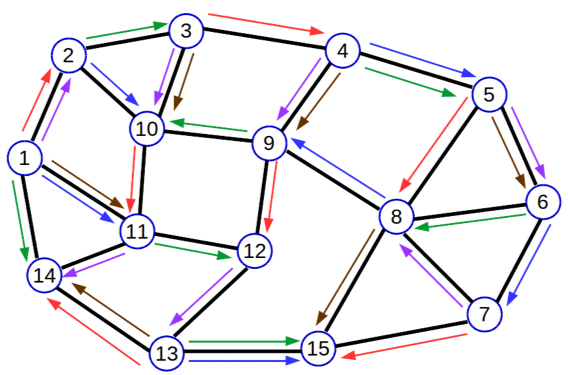
\includegraphics[scale=0.90]{Images/mesh.png}
		\end{center}
	\end{adjustwidth}
	\caption{Mesh Network}
\end{figure}

\section{Objectives and Significance of the project} 

The project is divided into two phases, figuring out how to arrange the sensors into a mesh
and using some mesh arrangement of sensors for a yet to be determined application. The first half has
several portions. First, a means of communication for the network, current
consideration being Zigbee or Bluetooth 5. Then we must setup the sensors to communicate together to
a base station. Depending on the mesh protocol chosen, we must then figure out how to make the
network adaptive to a changing number of nodes. Finally, we must parametrize the system to
understand its limitations for when we choose an application later. We expect the application phase of
the project to be the bulk of said project. We have yet to decide on potential candidates yet.

The significance of the mesh network becomes clear in the application of the network. Some examples
provided by Kionix include the following: a blanket of accelerometers for shape detection, a line of
sensors to detect impact and deformation, or a plane of sensors that can provide information about a
covered object.
 
 	\begin{figure}[!h]
	
	\begin{adjustwidth}{-1.5cm}{}
		\begin{center}
			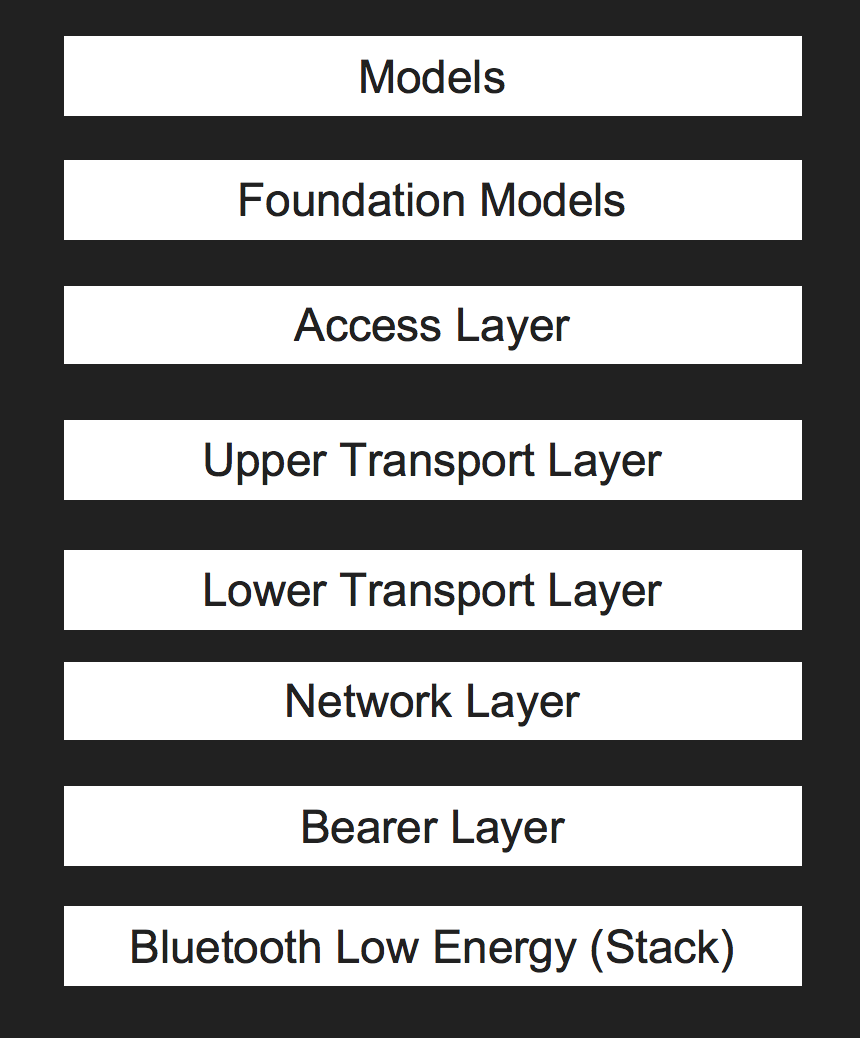
\includegraphics[scale=0.40]{Images/stack.png}
		\end{center}
	\end{adjustwidth}
	\caption{BLE Mesh Stack}
\end{figure}

 	\begin{figure}[!h]
	
	\begin{adjustwidth}{-1.5cm}{}
		\begin{center}
			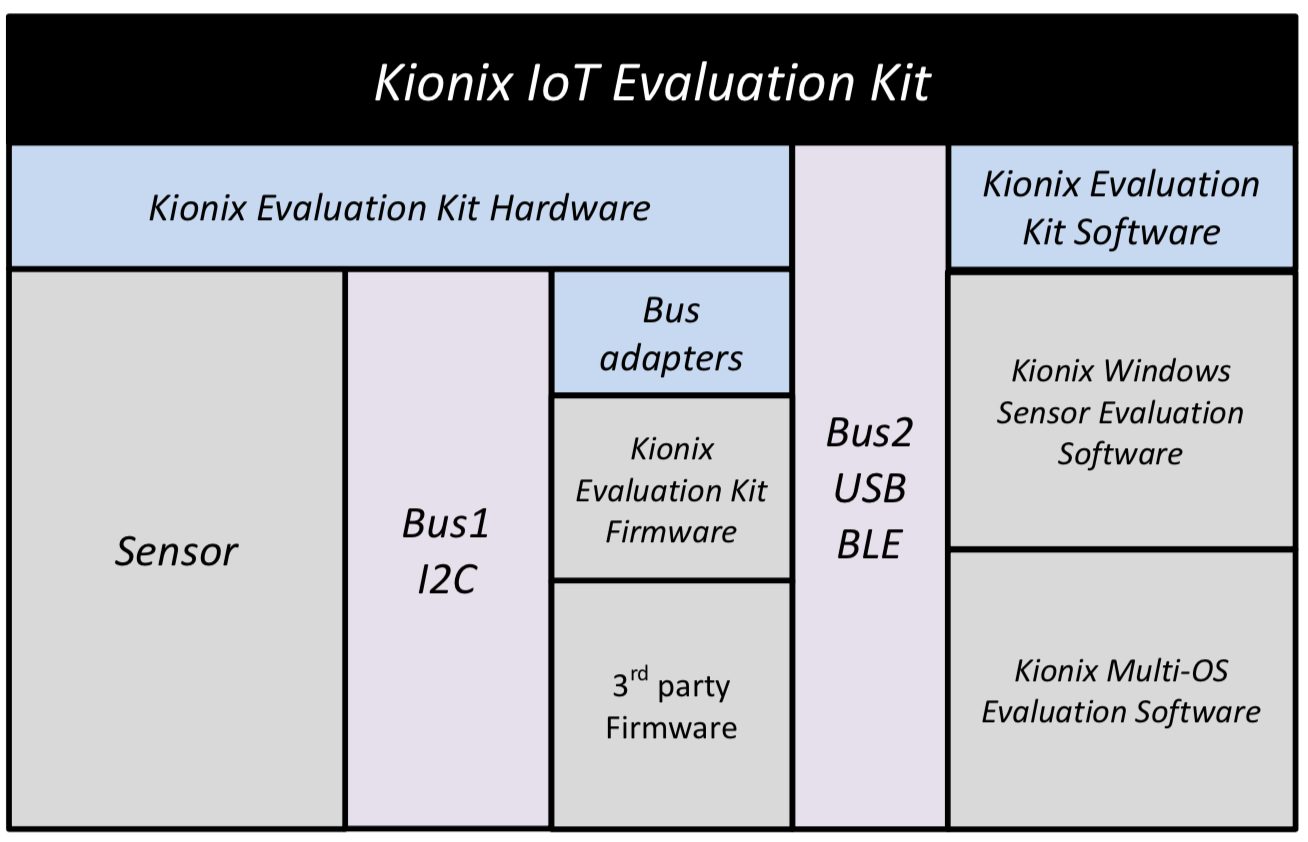
\includegraphics[scale=0.50]{Images/rokistack.png}
		\end{center}
	\end{adjustwidth}
	\caption{Kionix IoT Evaluation kit}
	\label{kionixstack}
\end{figure}

We chose to proceed with the BLE mesh as the Roki node uses the nRF52840 BLE 5 module. Zigbee has shown to be equally promising and we will continue to explore this option as well. From Fig. \ref{kionixstack}, we could flash our firmware into 3\textsuperscript{rd} party firmware module which could aid on chip processing.



\section{Progress}
This semester, our focus has been on exploring the problem space and the equipment that we are using, along with the technology provided to use by Kionix. We have also done research on mesh implementations, and Bluetooth 5.0, which will be using to implement the sensor mesh. Our progress is outlined more specifically below. We have been synthesizing our mesh research and Kionix sensor research by planning on reading multiple sensors at a time, and synthesizing the data. 

\subsection{RoKiX IOT Node}


\subsection{nrf Dev Boards}

\subsection{Integration of custom nrf firmware}

\subsection{Topology Visualization}

	\begin{figure}[!h]
	\begin{adjustwidth}{-1.5cm}{}
	\begin{center}
		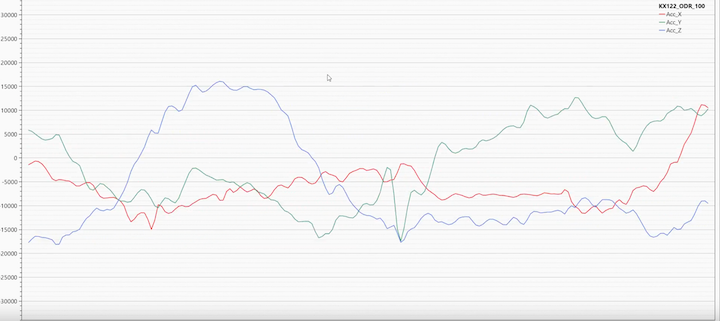
\includegraphics[scale=0.99]{Images/windowsgui}
	\end{center}
\end{adjustwidth}
\caption{Windows GUI Output}
\label{windowsgui}
\end{figure}

\section{Project Timeline}

The timeline below shows what parts the the project we hope to start and complete at which times. We plan on using the timeline below as a guide throughout the project, but it may change as we begin the technical work in the project. We have included the timeline as a table, and as a Gantt chart. \\
\\
Initially, our schedule for next semester included work on a wired RoKiX mesh, and we considered building a mesh out of Kionix sensors and BLE modules which we could purchase in large quantities. However, because Kionix is working on a project involving lower cost, smaller accelerometer nodes, and because a wired mesh would be limited, we have chosen to move forward with the Bluetooth 5.0 RoKiX mesh. We plan on experimenting with the processor embedded in the nodes, and running our own application code next semester as well, after discussing the accessibility of the RoKiX firmware. 
\\
\\


\subsection{Gantt Chart}
 

 	\begin{figure}[!htbp]

 \begin{adjustwidth}{-1.5cm}{}
\begin{center}
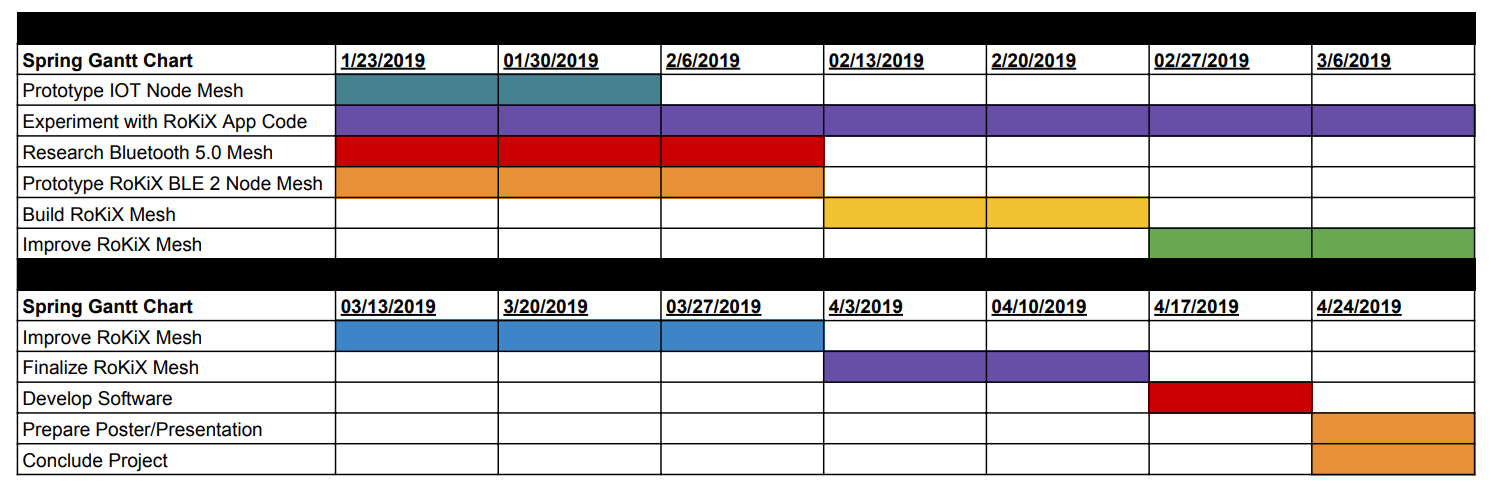
\includegraphics[scale=0.33]{Images/gantt.png}
\end{center}
 \end{adjustwidth}
\caption{Gantt Chart}
 	\end{figure}


%\section{Budget}

\section{Deliverables/ Goals for Spring 2019}
\begin{itemize}
	\item[] \textbf{Sensor Familiarization}
	\item Read Data from Kionix Sensor \cite{kionix}
	\item Communicate with multiple sensors simutaneously
	\item Determine Method for creating mesh network of Kionix sensors
	\item[] \textbf{Minimum Deliverable}
	\item Build a Roki Mesh Network
	\item[] \textbf{Wireless Familiarization}
	\item Read Data from Kionix Sensor wirelessly
	\item Communicate with multiple sensors simutaneously wirelessly
	\item[] \textbf{Preferred Deliverable}
	\item Build Wireless Mesh with auto-enroll
	\item[] \textbf{Additional Deliverables}
	\item Create software packages to analyze measurements for specific applications
	\item Create a scalable framework which can utilize mesh network for applications like herd tracking which would otherwise be limited by range.
	\item Create software front end
\end{itemize}

In the above list of objectives, first section includes tasks which we need to accomplish in order to understand the hardware and components that we are working with. Once we have an understanding of the components in our system, we will continue to produce the minimum deliverable for an acceptable project, the wired sensor mesh. After that objective, we will start to better understand the components that we need for a more complex project. Following that, we will deliver a more complex system, the wireless sensor mesh. If time permits, we will also deliver software to augment our system and provide automatic analysis of results. 



\section{Contributions}

\subsection{Mike}

This semester, I have contributed to the proposal, and to working with the Kionix nodes. During the beginning of the semester, I worked on the proposal by laying out the plan for the project. This involved taking the high level project statement and goals, and breaking them down into manageable, independent tasks. I relied on input from the team and our advisors to develop a plan that everyone was satisfied with. After determining what the goals for the project were, I sorted our plan by priority. I determined which goals led to a minimum deliverable, and which goals built upon the others, and organized them as such. I then developed a timeline which we would plan to follow as the project progressed. This involved estimating how much time each task would take, splitting the time that we had to fit these tasks, and ensuring that some time was left over in case I underestimated the amount of effort any of the tasks would require. I then added figures, and clearly listed the goals and schedule. 
I also worked on understanding the Kionix nodes we have been given. I explored the IOT node using all of the software Kionix supplied, and established a connection to read accelerometer data with the Windows GUI over Bluetooth and over serial. I also connected to the sensor using my own Linux system over serial and over Bluetooth, recording the necessary steps to do so along the way. I modified the Kionix command line software to read the sensor more easily for our use case, and plot the read sensor data on Linux as well as Windows. I have explored the IOT node Kionix command line tools in depth, and have developed a good understanding of many of the components and methods for communication. I have also read through many of the library functions provided by Kionix, which has helped my understanding as well. I also wrote a script to test reading two IOT nodes over Bluetooth on Linux, but did not have a chance to test it. I outlined the procedure to read the sensor over wired and wireless protocols to the Raspberry Pi using a similar procedure as when reading to Linux. I also established a serial connection to the RoKiX node, and determined where the software needs to be modified to allow Linux Bluetooth connection to the RoKiX node, after reading the documentation for the RoKiX node connections using Linux systems and the command line interface. I have been able to compare the IOT node command line interface with the RoKiX node interface, which has helped the group understand how communication with the RoKiX node works. I have also examined the process of reflashing the Kionix devices by reading through the documentation, and downloading the firmware and necessary tools.

\subsection{Kenneth}

Within a week after joining the Sensor Mesh Project group, I was tasked with doing research on Zigbee Networks to determine whether it would be a viable means for communication.  I looked at a few implementations and considered how we could apply it to our project. Shortly after we began drafting the proposal, from which I was assigned to write the abstract and objectives sections. The abstract is important as it gives the background and summarizes the goals of the project. It is the very first thing that a reader would see so I tried to simplify explanations as best as I could. The objectives and significance section describes loosely how we will approach our assignment by Kionix and why it matters. I said that the project could be divided into two parts, implementing the mesh and then using in some sort of application. The significance of the sensor mesh was in the large variety of applications it could be used in. Around halfway through the semester we were presented with the Kionix IOT evaluation node along with the software necessary to interface to it from a windows computer. I helped with figuring out how to connect the node to the computer. I also spent time reading the provided documentation regarding the node to figure out additional features. It became clear that Bluetooth 5 was the intended mesh networking system after we decided to use the RoKi node. The node itself however would not come until later, since it was a new product by Kionix and ROHM. To prepare for this I began looking into mesh networking protocols provided by Nordic for when the RoKi node would come. Just before the break it came time to prepare the presentation for 5010. This was a light task in which each group member made a subsection of slides. I made mine in turn and spoke during the beginning third of the presentation during the appropriate week. We were given the RoKi node during the first Friday of December.  Upon reading some documentation, I learned that it uses the nRF52840 SOC by Nordic, which in addition to Bluetooth 5, can handle Zigbee and Thread. Going forward I will see how Zigbee is used on this system.

\subsection{Karthik}
Even before joining the group, I had a clear idea about multi-hop mesh networking from prior work experience. I along with my team came up with the direction for the entire project. I suggested to experiment with the latest and trending mesh networking technologies which were ZigBee Mesh and BLE(Bluetooth Low Energy) 5. I contributed to the background work and existing research in the field of mesh networking for the proposal. I also contributed to the software (SDKs) and hardware requirements such as development boards which would be required for experimenting with mesh networking. I then aggregated and  compiled the entire report using Latex. I also explored the IOT node provided by Jacob. I interface the IOT node with Mac OS X and Android phone. I was even able to run the python CLI process to obtain the data on the terminal. This data was piped to a CSV file which could be used for data processing as mentioned in the plan for the spring semester. I also familiarized myself with the wired accelerometer sensor which was initially planed for a wired mesh. This idea was later abandoned as Kionix required a wireless prototype. After receiving the RoKi IOT node, I familiarized myself with nRF52840-DK firmware which has BLE 5 and mesh support. I setup the tool-chain and development environment for nrf mesh (proprietary Bluetooth mesh networking developed on BLE by Nordic Semiconductors). This can be uploaded to the RoKi node using the nordic Android app. I have also gone through the documentation of the new node to understand the SoC architecture which will be crucial in adding mesh firmware to the RoKi node. From Fig. \ref{kionixstack}, we could flash our firmware into 3\textsuperscript{rd} party firmware module which could aid on chip processing.

\section{Bill of Materials}
\begin{table}[h!]
	\begin{tabular}{|l|l|l|}
		\hline
		Component & Price Per Unit & Quantity \\ \hline
		KX123-1039 evaluation board & \$100 & 1 \\ \hline
		RoKi node & $\sim$ $30 - $50 & 2 \\ \hline
		Raspberry Pi 3B & \$35 & 1 \\ \hline
	\end{tabular}
\end{table}
\section {Conclusion}
Mesh networking is one of the first steps towards infrastructure-less and decentralizing networks. Mesh networking allows extraction of useful information from multiple sensors which would otherwise be impossible from a single data point. It's also a step in the right direction towards last mile connectivity and power savings. Moreover, with the advent of 5G ( fifth generation networks), multi-hop mesh networking has significant implications. We wish to aid Kionix with their applications.

\section{Contacts}

	\textbf{Joseph Skovira}:  jfs9@cornell.edu\\
	\textbf{Jacob George}  :  jgeorge@kionix.com
	
\section{Appendix}
\subsection{BLE 4 Mesh}
Since, the RoKi IOT node was delayed I started working on an architecture to make a mesh interface on top of BLE 4 stack. A BLE device has two basic modes: device discovery and connection mode. We alternate between these two modes to achieve a pseudo multi-hop network. When a node wants to send data, it updates the broadcast data accordingly and then broadcasts it. When a node is scanning and comes across a broadcast message sent by another node, it reads data from it and updates the data in its own advertisement and then broadcasts it. This accounts for one hop. By extending this, multi-hop communication can be achieved. This is can be further expanded during spring as a fallback plan. 
	
\bibliography{refer.bib} 
\bibliographystyle{ieeetr}


\end{document}

